%!TEX root = ../Thesis.tex
\chapter{Discussion}\label{cha:discussion}
%
\textcolor{red}{Here you should discuss all aspect of your thesis and project. How did the process work? Which choices did you make, and what did you learn from it? What were the pros and cons? What would you have done differently if you were to undertake the same project over again, both in terms of process and product? What are the societal consequences of your work?}

\section{Results}\label{sec:disc_results}
By studying the results from \autoref{cha:results} we see some interesting findings. A presentation of the results plotted with the video number on the x-axis can be found in \autoref{cha:appendix-video-rating}. Let's discuss some of our findings.

When we take a look at the first question of the subjective rating ("How satisfied are you with the quality of the silhouette extraction?") we see that video 4, 5 and 10 had the overall worst rating. The same applies for question 2 ("Did you notice any artefacts with the silhouette extraction?") and 3 ("Do you think the artefacts were annoying?")

We can also see that the three best videos from question 1, video 6, 9 and 12, also were the clear winners with the lowest level of noticeable artefacts and level of annoyance. While these videos were the clear winners from the subjective tests, it is not mirrored in the objective tests. 

Video 3 had the best objective score, but it was not popular in the subjective score. When we analyse this specific video closer we see what this might come from. This video has a few single bad frames with bad segmentation. While the objective scores does not penalise the single bad frames that much, it seems to be really annoying to watch for humans. Humans see these bad single frames as clear glitches and errors in the video. Some of the highest annoyance levels came from the videos with the best objective scores. 

The videos with the white wall performed overall better than all of the other backgrounds for the subjective measures, as expected (video 3, 6, 9 and 12). This is not the case for the objective measures, as there seems to be no clear pattern in which videos perform better than other. Sometimes the white wall background performed the best (video 3), and sometimes the window background performed the best (video 5 and 8).

Video 1, 2 and 3, where the person was showing an object, had almost the same rating for in the case of the subjective ratings. This was unrelated of the background. The results were not the worst either.

The levels of noticeable artefacts seems to be pretty linear with the level of annoyance for each video. There were no extreme cases where the participants thought the level of artefacts did not impact the perceived quality of the silhouette extraction.

We also notice something interesting with the dark and light clothing. The dark clothing, video 4, 5 and 6, got a overall much better rating objectively than the white clothing. But, when we look at the subjective rating, the light clothing got a much better score. One final interesting note, is that the dark and light clothing performed almost equally good objectively with the white wall background (video 5 and 8).

As far as we can see, there is no clear connection between the objective measures and the subjective measures, meaning none of our supporting hypothesis of our research questions were correct. The best subjectively rated videos, was overall not greatly rated objectively and vice versa.


\section{Quality of Experience}\label{sec:disc_qoe}

As already mentioned in \autoref{sec:previous} the measure of Quality of Experience can be a cumbersome task. Quality of Experience is by itself very subjective, up to each personal users viewpoint and relationship to whats in question. 

The perceived level of ''good quality'' varies in a large extent from person to person. We can ask ourselves what even is quality of experience? How would we be able to measure this in a way when each experience is so individual for each human being. 

There is no single scalar value which can be put to this. Only what we as human feel ourselves. The subjective rating results presented in this thesis has no definite answer, and it is up to each reader to evaluate with themselves if they think the results were sufficiently good enough to put the label of a high quality of experience on it. 


\section{The videos}\label{sec:disc_videos}

With the limited time frame and level of resources in such a thesis, only a selected number of test videos could be performed. By extending the number of videos to represent a larger number of use cases and variations, we could be able to get a more representative result on the level of quality of the \acrlong{mlbfe}. 

The constructed videos were constructed of foreground videos with a white male in his twenties representing a very small number of people which will be able to use this technology in the future. The different background videos were also constructed to represent some different challenges for the algorithm to work with, but they are not very representative of the final ''backgrounds'' that's going to be used in the field. One can imagine that the final users will more often than not film themselves in their living rooms, and not at a university campus. 

The videos did also not present other scenarios which one could imagine would be challenging. To name a few – Different types of lighting, picking up objects, more movement in the background, several people in the frame and outdoor filming. 

Another small thing to note, is that because of the green screen setup, we were unable to film a full body. This resulted in videos where the person had its feet cut off, and this might not be representative of the final use cases where most likely the entire bodies of the in frame persons will be used. 

While the placement of the ring lights were decided by trial and error to minimise shadow casting, we saw that this could have been improved in the chroma-key editing. Some of the videos had some shading issues, leading to a not entirely perfect chroma-key deletion. This was accounted for by adjusting the settings, giving pretty decent results despite of the shadowing. The shadow casting might give us a wrong ground truth since the silhouette will be bigger and not perfectly covering only the body of the person in the frame. Because of this, it might happen that the \acrshort{mlbfe} will perform better than the chroma-keying, but the objective rating will be penalised since it will see the machine learning cutting too much of the silhouette. The shadowing problem could be solved with improved lighting, either by using more lights or use other lighting technique. 

\section{Subjective Testing}\label{sec:disc_subjective}

The subjective testing in this thesis was done using a web form run through Google Forms. This was done as the view was that it was more important to get a larger amount of data, than what would have been possible by a physical survey. As this thesis also was done the fall of 2021, the Corona pandemic was still a part of our every day, making it even harder to recruit people to do physical testing. By using Google Forms we made an easy and readily available survey that could easily be shared with a lot of people. Because of this we got a good number of participants for the survey. 

But doing the testing via a web survey also introduces a lot of new influencing factors. Since the form was sent directly to the participants, the participants were able to do the survey in an uncontrolled environment. System influencing factors and context influencing factors can play a huge role here. We have no way of knowing what type of device the participants were using. Some probably used their phones, some used their computers, all having different screen sizes and screen technology. This could influence the entire viewing experience and the total experience, 

Since the participant were able to do the questionnaire when and where they wanted, we do not how the context influencing factors affected them, such as location, time of day, interruption's and so on. 

The only possible way to put a video into the Google Forms, was to use Google's own video hosting service, YouTube. As mentioned in \autoref{sec:system_subjective} the videos were uploaded unlisted to a newly created account to minimise targeted recommendations and other pitfalls in the YouTube algorithm. Using simple YouTube videos, we have no way of controlling whether or not the participants saw the videos only once or multiple times. The participants could also have seen the video as is in the forms, watched it in full screen, watched the video in a new tab within YouTube's own website and therefore seen lots of other video suggestions. Again a lot of influencing factors which can have impacted the general experience of the user. 

The result may also be biased because of the demographic and human influencing factors. The vast majority of the participants were higher educated, and within the educated a majority of the science of technology. By looking at \autoref{fig:age}, one could argue the age was not very evenly distributed. The age group from 18 to 34 were highly represented, but the other groups had a varied representation. The age distribution from this testing might not be a good representation of the final user base of this technology. 

The order of how the videos would be presented was also randomised by a Python function. This was done to prevent the participants to see the same foreground videos after one another, but one could ponder if the order of the videos should be carefully selected or not. Maybe all of the same foregrounds, or the same backgrounds, should be presented after each other? Could this have given a completely different result?

\section{Subjective VS Objective}\label{sec:disc_qua}

We decided to try to measure both subjective and objective data for this thesis, as it was not given that only one of them would give a clear result on the actual quality of the \acrlong{mlbfe}. 

During EPFL's development, they used similar objective testing like we have done in this thesis, to evaluate the technology. But since the final product will be used by real humans, the objective testing would not be quite representative of the final user experience. That is why we decided to go for both types of evaluations, to ensure a more representative result to the end use case, and to see if the objective and quantitative measures could yield a result with a matching pattern for the subjective and qualitative testing.

In our final inspection of the result, it seems like we are unable to find any particular pattern between the objective measures, \acrshort{iou}, \acrshort{dc} and \acrshort{pa}, and the subjective measures of satisfaction, level of artefacts and level of annoyance in the \acrlong{mlbfe}, as discussed in \autoref{sec:disc_results}. This further enhances our claim of needing both the objective and the subjective measures. The objective measures might work better for evaluating the quality at a single frame level, while the subjective measures might work better for the evaluation of the entire video itself. 

The objective measures gives us an image of how each single frame gets segmented, but the average result of this measure, does not give a clear result. To better utilise the objective measures, one should use an another way of presenting the final result than the average, as the extremes gets crushed by the other good performing frames. 

The subjective measures reflects the extremes clearer as the videos with single bad frames spread in the video got a bad rating. The single sporadic bad frames, of an otherwise good segmented video, impacted the participants quality of experience in a more profound way than the videos with smaller extremes, but overall might have had a weaker objective score. 

To combat this, the machine learning model could maybe implement ways to get rid of the extremes. For example – In the testing used in this thesis, the extremes were single bad frames. These single bad frames could maybe be digitally manipulated to match the surrounding frames. In video 3, where the person held a book, frame 256, seen in \autoref{fig:256}, had a \acrlong{fpn} score of $20505$, while the previous frame, seen in \autoref{fig:255}, had $12723$, and the following frame, seen in \autoref{fig:256}, had $13071$. If the machine learning model had done an automatic content aware filling for the missing book in frame 256, the subjective measure might have suffered less, as the seemingly glitch would have been less prominent

\begin{figure}
\centering
\begin{subfigure}{.3\textwidth}
  \centering
  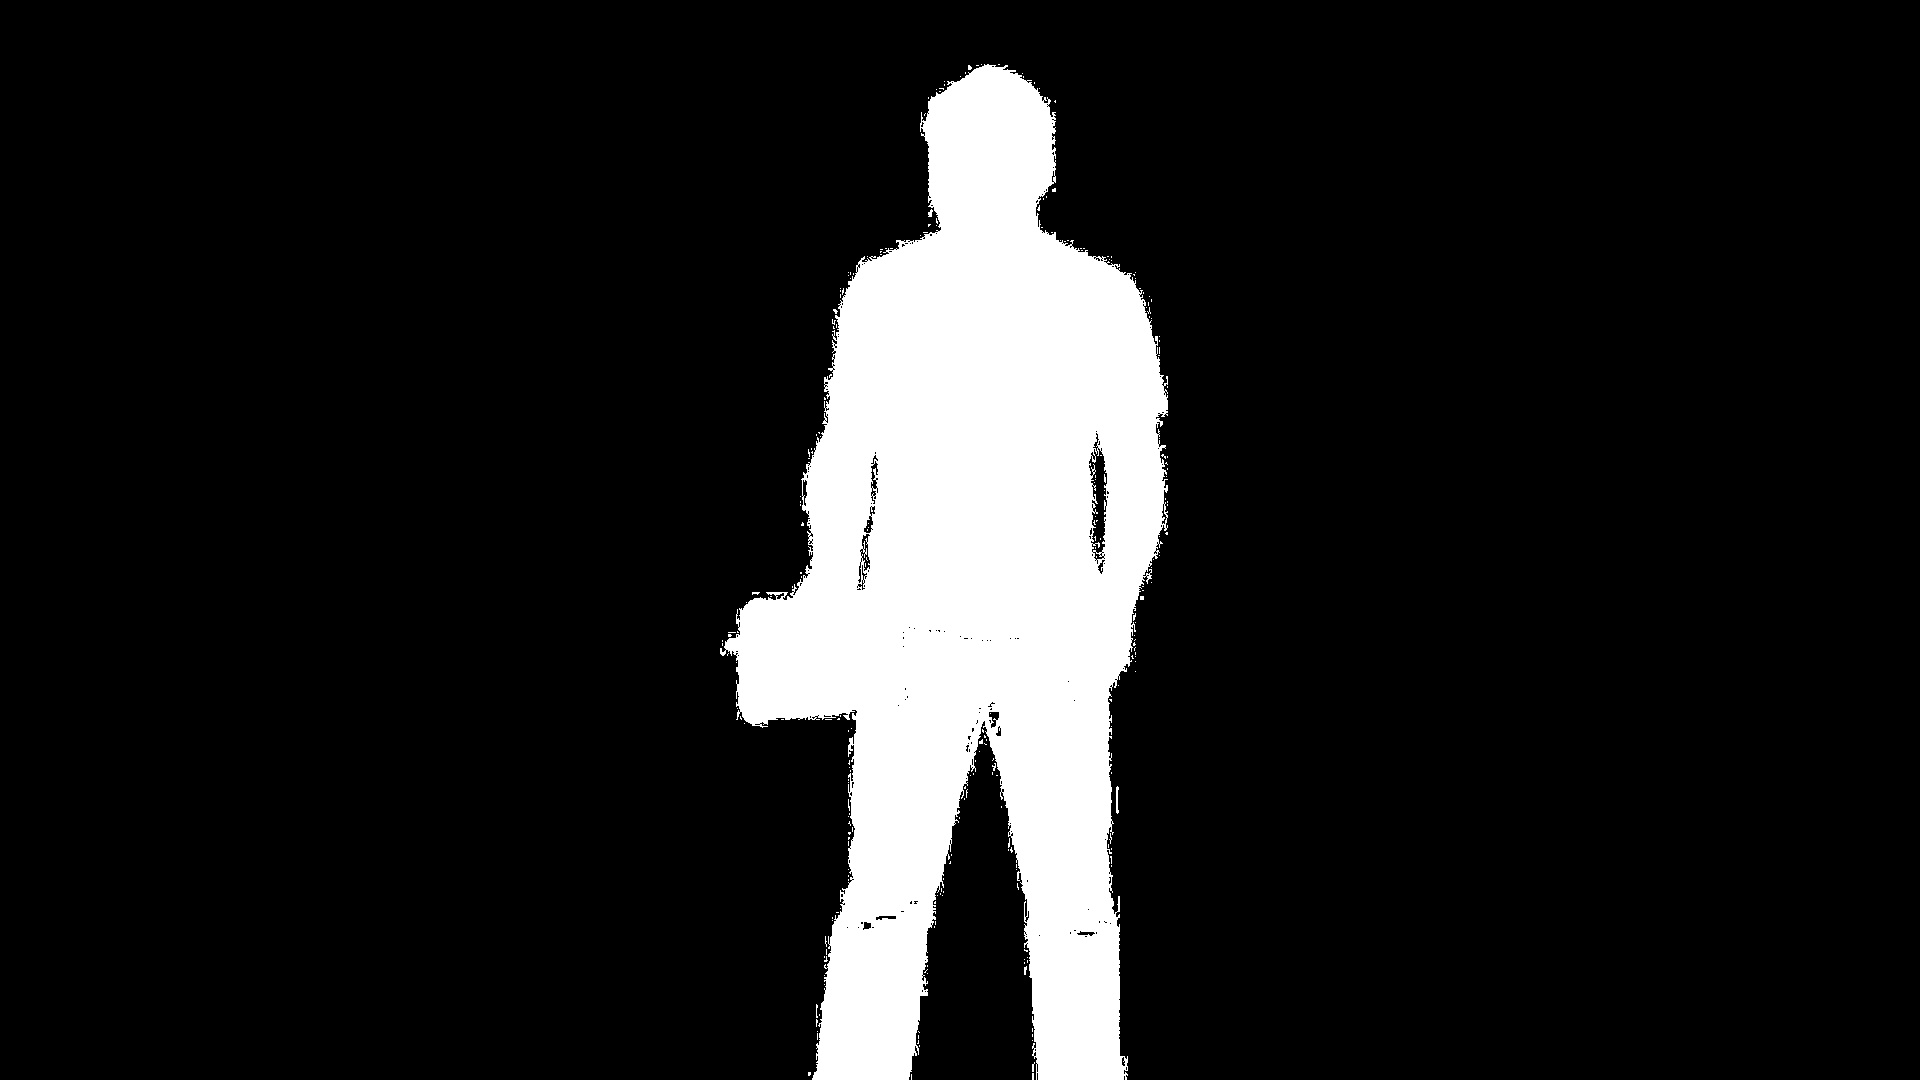
\includegraphics[width=\linewidth]{img/256/FG_Showing-Object_BG_White-Wall_fg_255.jpg}
  \caption{Frame 255 of video 3}
  \label{fig:255}
\end{subfigure}%
\begin{subfigure}{.3\textwidth}
  \centering
  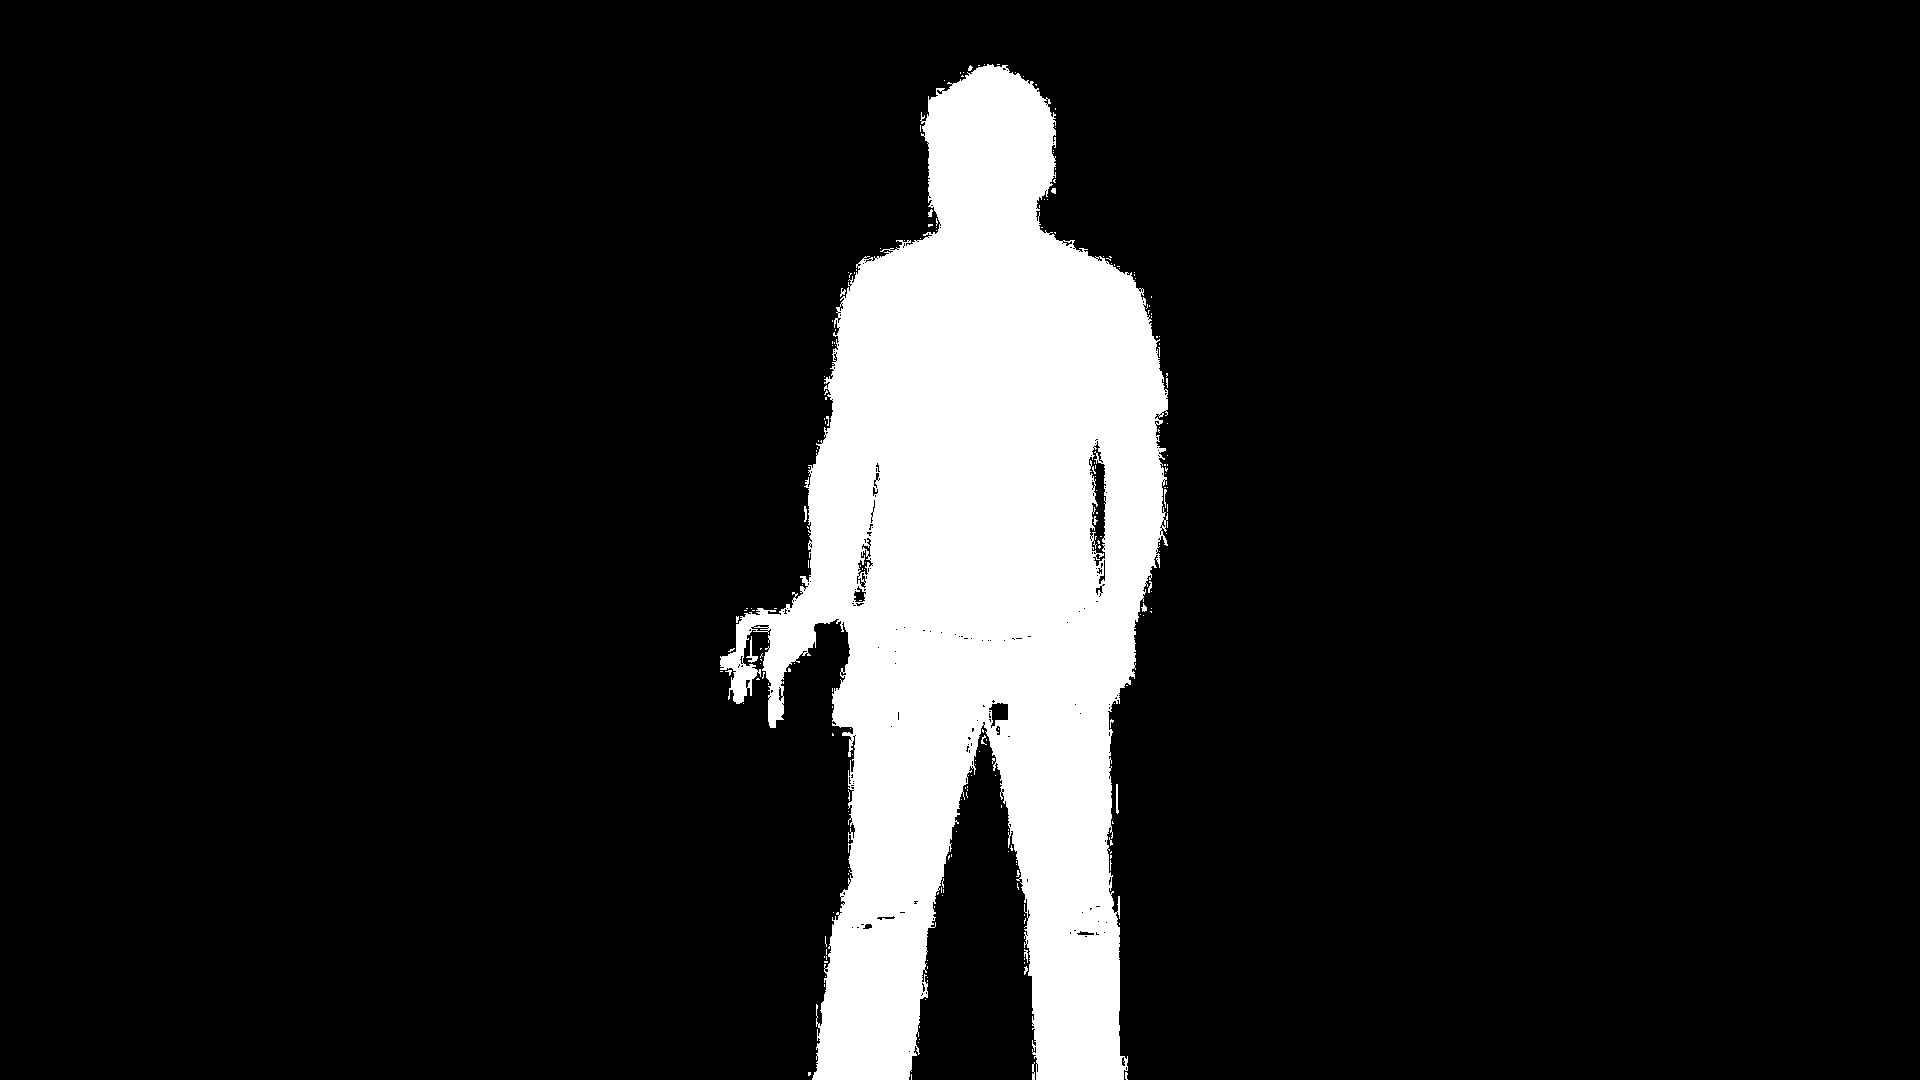
\includegraphics[width=\linewidth]{img/256/FG_Showing-Object_BG_White-Wall_fg_256.jpg}
  \caption{Frame 256 of video 3}
  \label{fig:256}
\end{subfigure}%
\begin{subfigure}{.3\textwidth}
  \centering
  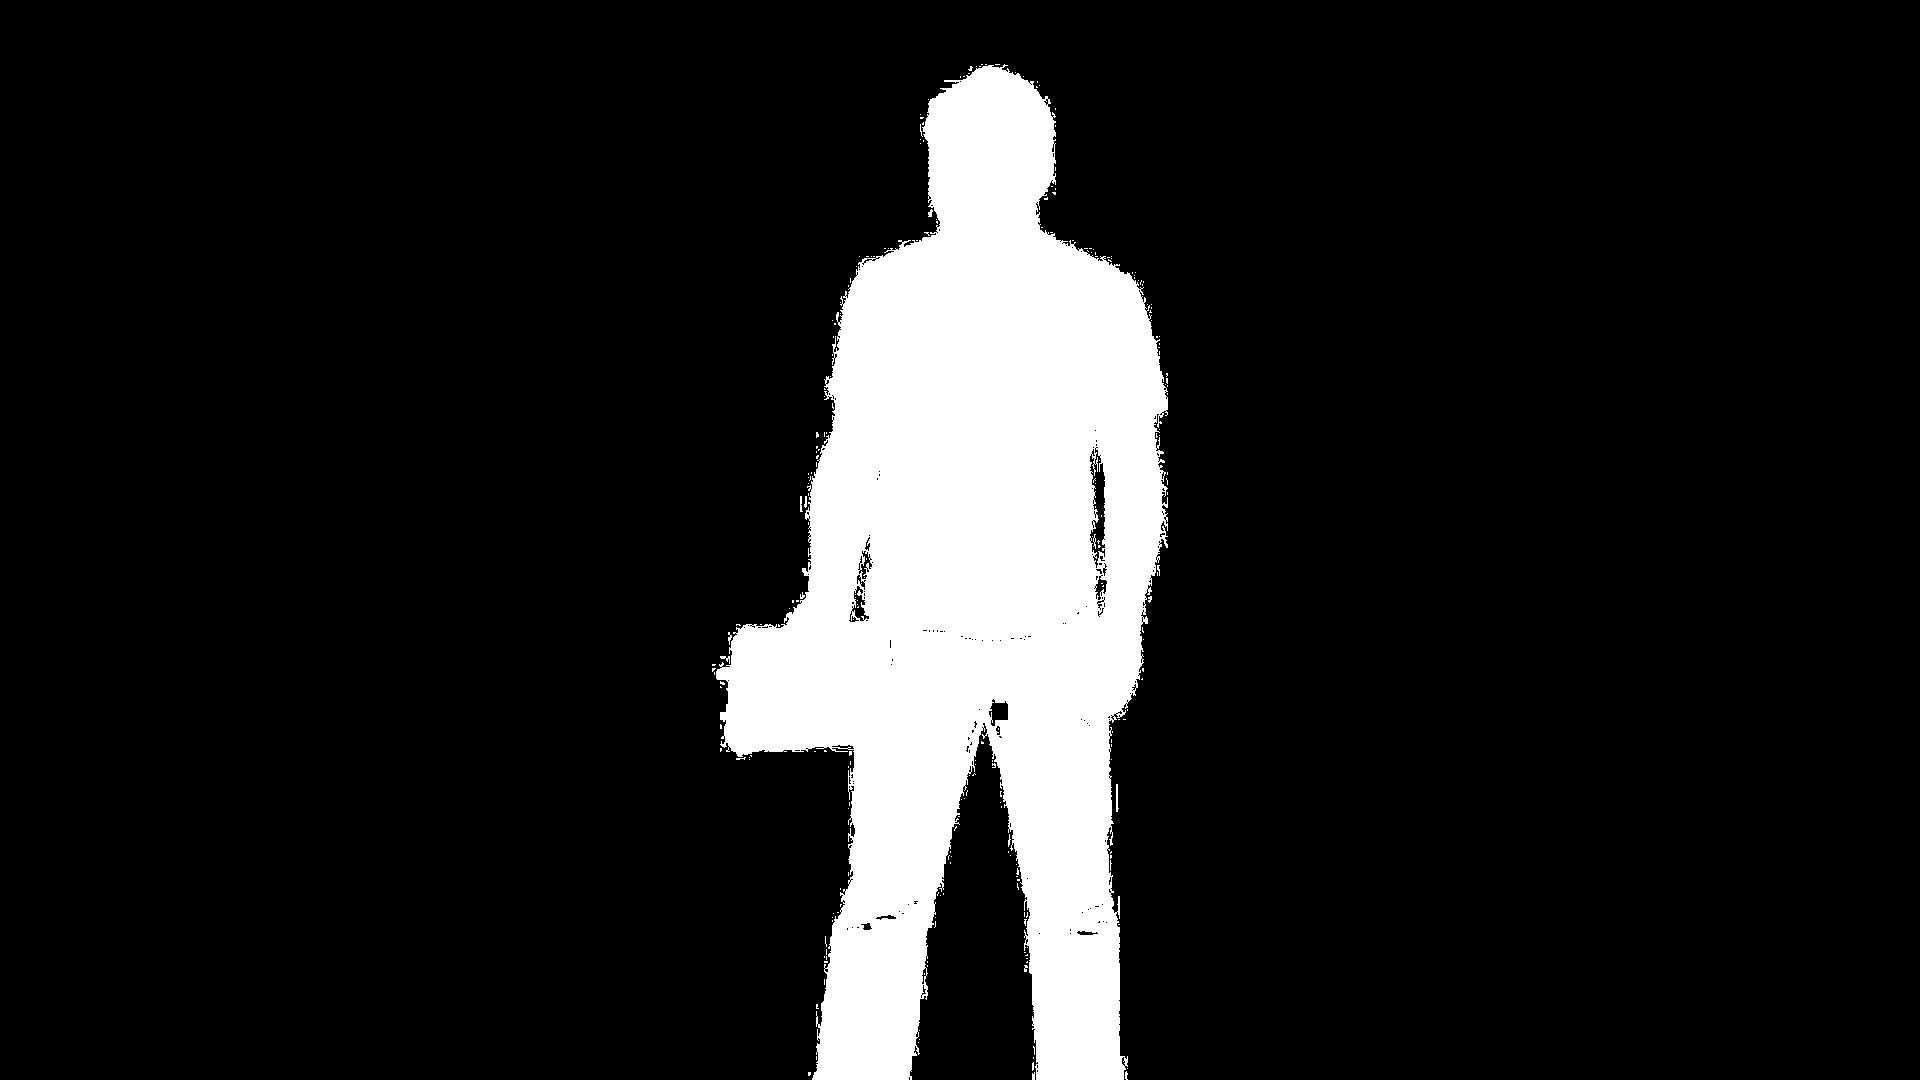
\includegraphics[width=\linewidth]{img/256/FG_Showing-Object_BG_White-Wall_fg_257.jpg}
  \caption{Frame 257 of video 3}
  \label{fig:257}
\end{subfigure}
\caption{Show case of a single bad frame}
\label{fig:single_bad_frame}
\end{figure}

Another interesting note, also discussed a bit in \autoref{sec:disc_results}, was the difference in results of the dark and light clothing. This further highlights the different outcomes of the objective and subjective measures, where the dark clothing got a better rating objectively than the white, but the subjective rating yielded a better score for the light clothing. By manually comparing the dark clothing videos to the light clothing videos, there seems to be little difference between them. It could be interesting to see how the results would turn out if the background colour was a different colour than black. With the black clothing, it could maybe be difficult to distinguish the silhouette from the background. Maybe if the background was for example a typical bright green screen green, it would have yielded different results subjectively, since the silhouette could possibly be easier to separate from the background. 

\section{Data set}\label{sec:disc_data}
The \acrlong{mlbfe} model has been trained with the data set from \cite{gmnu21}, further elaborated in \autoref{sec:training}, and while this is a general data set for separating human silhouettes in the foreground from what ever background, one can wonder if this data set representing a wide enough data set preparing the model for all of the final use cases. 

In our testing, we specifically saw that the current model with its training struggled a bit with foreign objects in the foreground scene. Like with other machine learning models, it is often not the technology itself which is the weakness, but the amount of data which the model has been trained and validated on. To increase the performance, an increased size of the data set used for training might be beneficiary. 